\section{Zone Internal Gains }\label{zone-internal-gains}

\subsection{Sources and Types of Gains}\label{sources-and-types-of-gains}

Internal heat gains from lights, people, and equipment of various types are often significant elements in the zone thermal balance.~ EnergyPlus allows the user to specify heat gains for several equipment types including people, lights, gas/electric equipment, and several other types.~ The total heat gain is comprised of convective, radiant and latent gains in various proportions from these sources.~ Convective gains are instantaneous additions of heat to the zone air.~ Radiant gains are distributed on the surfaces of the zone, where they are first absorbed and then released back into the room (with some fraction conducted through the surface) according to the surface heat balances. \{See Surface Heat Balance Manager / Processes in this document\}.~ Latent gains must be handled by ventilation or air conditioning equipment.~ Recommended heat gains are given by ASHRAE {[}1{]}.~ These recommendations include the sensible (convective plus radiative) and latent proportions.~ Sensible gains from equipment are primarily radiant.~ The user can specify the heat gains and proportions for any type of equipment.~ Determining the gains from lights, people and baseboard heat are slightly more complicated.

\subsection{Heat Gain from Lights}\label{heat-gain-from-lights}

The input object Lights provides a model for internal gains from lights.~ Radiant gains from lights must be handled differently from other radiant gains for reasons described here (long wavelength description).~ The total radiant gains from lights must be divided into visible and thermal portions.~ For example, the total electric input to typical incandescent lights is converted to 10\% visible radiation, 80\% thermal radiation, and 10\% convective gain.~ In contrast, the electric input to typical fluorescent lights is converted to 20\% visible radiation, 20\% thermal radiation, and 60\% convective gain {[}2{]}.~ These percentage splits are under user control with the Lights input object.

\subsection{Heat Gain from People}\label{heat-gain-from-people-000}

The input object People provides a model for internal gains from occupants.~ Heat is generated in the human body by oxidation at a rate called the metabolic rate (see Thermal Comfort discussion for more details).~ This heat is dissipated from the body surface and respiratory tract by a combination of radiation, convection, and evaporation.~ The relative proportions of sensible (radiation plus convection) and latent (evaporation) heat from people is a complex function of the metabolic rate and the environmental conditions.~ EnergyPlus uses a polynomial function to divide the total metabolic heat gain into sensible and latent portions.~ That function is based on a fit to data {[}3{]} at average adjusted metabolic rates of 350, 400, 450, 500, 750, 850, 1000 and 1450 Btu/h each at temperatures of 70, 75, 78, 80, 82 degrees Fahrenheit.~ Sensible gains of 0 at 96 F and sensible gains equal to the metabolic rate at 30 F were assumed in order to give reasonable values beyond the reported temperature range.

Average adjusted metabolic rate {[}3{]} is the metabolic rate to be applied to a mixed group of people with a typical percent composition based on the following factors:

\begin{itemize}
  \item Metabolic rate, adult female = Metabolic rate, adult male X 0.85
  \item Metabolic rate, children = Metabolic rate, adult male X 0.75
\end{itemize}

The original data was in I-P (Inch-Pound) units, but the following correlation is in SI (Systems-International) units.

\begin{equation}
  \begin{array}{ll}
    S &= 6.461927 + .946892 M + .0000255737 M^2 + 7.139322 T - .0627909 T M \\
      &+ .0000589172 T M^2 - .198550 T^2 + .000940018 T^2 M - .00000149532 T^2 M^2
  \end{array}
\end{equation}

where

M = Metabolic Rate (W)

T = Air Temperature (C)

S = Sensible Gain (W)

Latent Gain is simply the total gain (metabolic rate) -- sensible gain:

\begin{equation}
LatentGain = MetabolicRate - SensibleGain
\end{equation}

\begin{figure}[hbtp] % fig 259
\centering
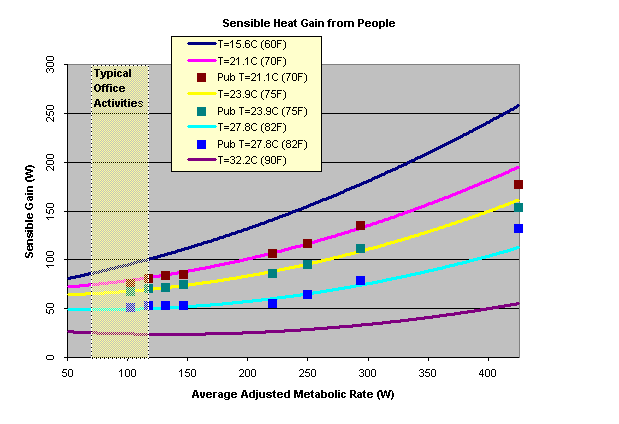
\includegraphics[width=0.9\textwidth, height=0.9\textheight, keepaspectratio=true]{media/image5820.png}
\caption{Sensible Heat Gain from People Correlation \protect \label{fig:sensible-heat-gain-from-people-correlation}}
\end{figure}

The function for sensible gain calculation is compared to the original data points in the following figure.~ The radiant fraction of the sensible gain is a user input on the People object.

\subsection{Heat Gain from IT Equipment}\label{heat-gain-from-it-equipment}

The input object ElectricEquipment:ITE:AirCooled describes air-cooled electric information technology equipment (ITE) which has variable power consumption as a function of loading and temperature. The calculations are described below.

\subsubsection{Variable Definitions -- User Inputs:}\label{variable-definitions-user-inputs}

\begin{itemize}
\tightlist
\item
  PDesign = Design power input when fully loaded and entering air temperature is at the user-specified design inlet temperature {[}W{]}
\item
  PFanFracDesign = Design fan power input fraction of total power input when fully loaded and entering air temperature is at the user-specified design inlet temperature
\item
  SchDesignLevel = Scheduled fraction of this equipment which is powered up
\item
  SchCPULoading = Scheduled fraction of CPU loading
\item
  TAirInDesign = Air inlet temperature at design condition {[}C{]}
\item
  VAirDesign = Air volume flow rate at design condition {[}m3/s{]}
\item
  VAirfLoadTAir = Air volume flow rate modifier function of TAirIn and SchCPULoading
\item
  PCPUfLoadTAir = CPU power input modifier function of TAirIn and SchCPULoading
\item
  PFanfFlowFrac = Fan power input modifier function of air flow fraction
\item
  RecircFracDesign = Recirculation Fraction at design condition {[}C{]}
\item
  RecircfLoadTAir = Recirculation Fraction modifier function of TAirSupply and SchCPULoading
\item
  UPSEfficDesign = Design electric power supply efficiency
\item
  UPSEfficfPLR = Electric power supply efficiency function of part load ratio
\item
  UPSLossFracToZone = Fraction of electric power supply losses to zone
\end{itemize}

\subsubsection{Variable Definitions -- Simulation Inputs:}\label{variable-definitions-simulation-inputs}

\begin{itemize}
\tightlist
\item
  TAirIn = Air inlet temperature at current conditions {[}C{]}
\item
  TAirSupply = Supply air node temperature at current conditions {[}C{]}
\item
  TZone = Zone air temperature at current conditions {[}C{]}
\item
  TRoomAirNodeIn = Room air model inlet node air temperature at current conditions {[}C{]}
\item
  RhoAir = Air density {[}kg/m3{]}
\item
  CpAir = Air specific heat {[}J/kg-K{]}
\end{itemize}

\subsubsection{Variable Definitions -- Intermediate Calculations:}\label{variable-definitions-intermediate-calculations}

\begin{itemize}
\tightlist
\item
  PCPUDesign = Design CPU power input when fully loaded and entering air temperature is at the user-specified design inlet temperature {[}W{]}
\item
  PFanDesign = Design fan power input when fully loaded and entering air temperature is at the user-specified design inlet temperature {[}W{]}
\item
  UPSPLR = Electric power supply part load ratio (can be greater than 1.0)
\end{itemize}

\subsubsection{Variable Definitions -- Outputs:}\label{variable-definitions-outputs}

\begin{itemize}
\tightlist
\item
  PCPU = CPU power input {[}W{]}
\item
  PFan = Fan power input {[}W{]}
\item
  PUPS = Electric power supply net power input {[}W{]}
\item
  TAirOut = Air outlet temperature {[}C{]}
\item
  VAir = Air volume flow rate {[}m3/s{]}
\item
  FlowFrac = Air volume flow rate fraction of design flow rate
\item
  RecircFrac = Recirculation fraction
\item
  QAir = Air cooling rate {[}W{]}
\item
  QUPS = Electric power supply heat loss rate to zone {[}W{]}
\item
  QConv = Convective heat gain rate to zone heat balance {[}W{]}
\item
  SHI = Supply heat index
\item
  SHIZone = Zone average supply heat index
\end{itemize}

\subsubsection{Calculations}\label{calculations}

The design power input is first split into portions for the CPU (everything in the equipment except the cooling fans) and the fan(s).

PCPUDesign = PDesign * (1 - PFanFracDesign)

PFanDesign = PDesign * PFanFracDesign

For each time step,  the air inlet and outlet temperature is calculated depending on the type of air flow calculation method. Considering data centers are different from normal well-mixed zones due to the uneven air distribution, two methods are implemented to calculate the IT inlet temperature and zone return air temperature, FlowFromSystem and FlowControlWithApproachTemperatures. Specifically, the IT inlet temperature differs from AHU supply air temperature, and the actual AHU return air temperature differs from the regular return air temperature when the zone is well mixed.

When using FlowFromSystem, the zone is assumed to be well-mixed. The air inlet temperature is calculated depending on the type of air node connection.

TAirIn:

\begin{itemize}
    \tightlist
  \item
    If Air Node Connection Type = AdjustedSupply
    \begin{itemize}
      \item RecircFrac = RecircFracDesign \* RecircfLoadTAir(SchCPULoading TAirSupply)
      \item TAirIn = TAirSupply \* (1 – RecircFrac) +TAirZone \* RecircFrac
    \end{itemize}
  \item
    If Air Node Connection Type = ZoneAirNode
    \begin{itemize}
      \item   TAirIn = TAirZone
    \end{itemize}
  \item
    If Air Node Connection Type = RoomAirModel
    \begin{itemize}
      \item TAirIn = TRoomAirNodeIn
    \end{itemize}
\end{itemize}

Using the air inlet temperature, the CPU power consumption, air flow rate, fan power consumption, and power supply power consumption are calculated.

PCPU = PCPUDesign * SchDesignLevel * PfLoadTAir(SchCPULoading, TAirIn)

FlowFrac = VAirfLoadTAir(SchCPULoading, TAirIn)

VAir = VAirDesign * FlowFrac

PFan = PFanDesign * SchDesignLevel * PFanfFlowFrac(FlowFrac)

UPSPLR = (PCPU + PFan) / (PCPUDesign + PFanDesign)

PUPS = (PCPU + PFan) * (1 - UPSEfficDesign * UPSEfficfPLR (UPSPLR))

The convective heat gain to the zone and the air outlet temperature are then calculated. The user specified fration of power supply losses are always added to the general zone heat balace convective heat gain. For air node connection types AdjustedSupply and ZoneAirNode, the CPU and fan power consumption are also added to the zone convective heat gain. For air connection type RoomAirModel, the gains from the CPU and fan power consumption are added to the outlet room air model node.

QAir = PCPU + PFan

QUPS = PUPS * UPSLossFracToZone

QConv:

\begin{itemize}
    \tightlist
  \item
    If Air Node Connection Type = AdjustedSupply OR ZoneAirNode
    \begin{itemize}
      \item   QConv = QAir + QUPS
    \end{itemize}
  \item
    If Air Node Connection Type = RoomAirModel
    \begin{itemize}
      \item   QConv = QUPS
    \end{itemize}
\end{itemize}

TAirOut = TAirIn + QAir / (VAir * RhoAir * CpAir)

The individual ITE supply heat index is calculated as shown below.

SHI = (TAirIn -- TAirSupply) / (TAirOut - TAirSupply)

The zone average ITE supply heat index is weighted by the air flow rate of each ITE object.

SHIZone = ∑ {[}VAir * (TAirIn -- TAirSupply){]} / ∑ {[}VAir * (TAirOut - TAirSupply){]}


If FlowControlWithApproachTemperatures is chosen, Two indices are introduced to represent the deviation: (1) Supply approach temperature ($\delta T_{supply}$) and (2) Return approach temperature ($\delta T_{return}$). The two temperature differences indicate to what degree the air flow management of data centers affects the air distribution, and how much they deviate from the regular well-mixed zone scenario.

$\delta T_{supply}=T_{in}-T_{supply}$

$\delta T_{return}=T_{return}-T_{return-mixed}$

Where, 

$T_{in}$: IT equipment inlet temperature

$T_{supply}$: AHU supply air temperature

$T_{return}$: The actual AHU return air temperature

$T_{airzone}$: The calculated zone air temperature (or return air temperature) if the room is well-mixed

The two approach temperatures can be calculated by CFD tools for typical IT load levels and air flow management of data centers, or provided by measurement data or lookup tables. 

It should be noted that, when FlowControlWithApproachTemperatures is chosen, 

(1) The inputs of Air Inlet Connection Type, Design Recirculation Fraction and Recirculation Function of Loading and Supply Temperature Curve Name are ignored.

(2) For multiple ITE objects defined for one zone, the same calculation method should apply. 

(3) Other return air heat gains from window or lights are not allowed when FlowControlWithApproachTemperatures is chosen.

(4) Apart from a single VAV terminal unit, other HVAC systems do not apply this method in the ITE zone.

When FlowControlWithApproachTemperatures method is applied, during sizing and simulation, as the zone is assumed to be unevenly distributed, the supply air flow rate is calculated as:

${\dot m_{sys}} = {Q_{sys}}/({C_{p,air}} \cdot ({T_{in}} - {T_{return}}))$,

where $T_{return}$ is the weighted return air temperature from all ITE objects in the zone. 

In this case, in the controlled zones with ITE objects, unlike the original thermostat setpoint control logic, the well-mixed zone temperature is not controlled. The actual controlled object is the supply air temperature. So when using this method, the user input of zone cooling setpoint is ignored and the unmet hour for cooling does not apply.

\subsection{Heat Gain from Baseboard Heat}\label{heat-gain-from-baseboard-heat}

The input object ZoneBaseboard:OutdoorTemperatureControlled provides a model for an outdoor temperature controlled baseboard heater that adds energy to the zone according a control profile as shown in the following figure.~ At TA = T2, the baseboard heat gain is Q2.~ For TA \textgreater{} T2, there is no heat gain.~ For TA \textless{} T1, a maximum amount of energy, Q1, is added to the zone.~ There is proportional control between those two temperatures:

\begin{figure}[hbtp] % fig 260
\centering
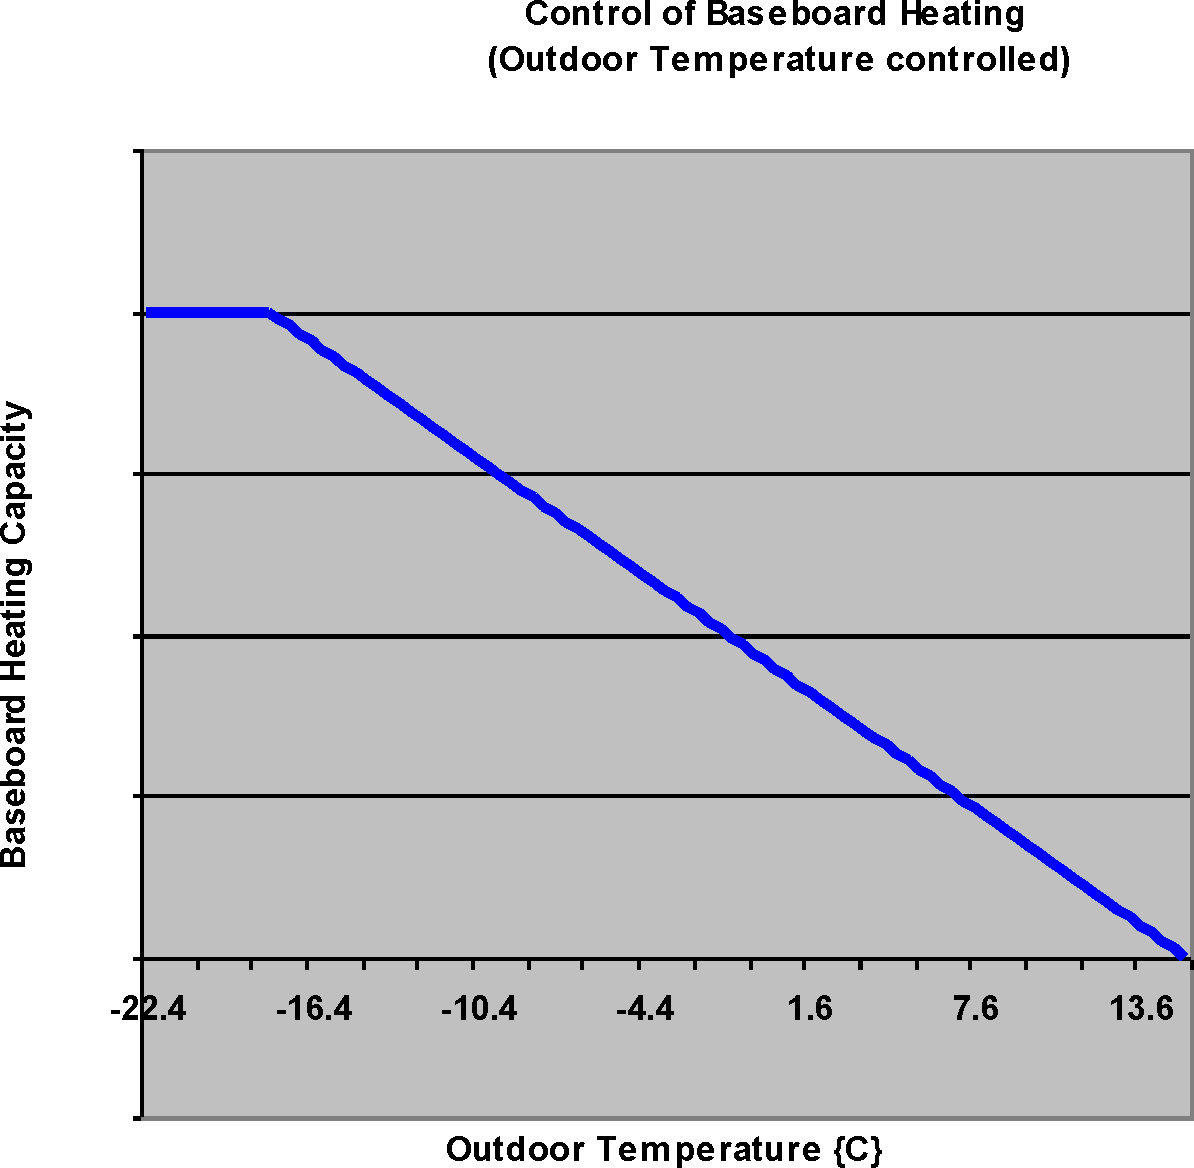
\includegraphics[width=0.9\textwidth, height=0.9\textheight, keepaspectratio=true]{media/image5821.png}
\caption{Control of Outdoor Temperature Controlled Baseboard Heat \protect \label{fig:control-of-outdoor-temperature-controlled}}
\end{figure}

\begin{equation}
Q = Q2 - \frac{{(Q2 - Q1)\cdot (T2 - TA)}}{{(T2 - T1)}}
\end{equation}

These temperature and capacity fields can be autosized based upon envelope, infiltration, and ventilation loads. To autosize these fields, users may set a design zone heating temperature that is assumed to be 20°C if blank.

The capacity at low temperature is the maximum capacity of the unit. It includes external envelope conduction load, infiltration load, and ventilation load in a space where the unit serves. The model first finds the lowest outdoor air temperature throughout design days included in the simulation, and determines the conduction load through external envelop as:

\begin{equation}
{q_{Cond}} = UA\left( {{T_{Htg}} - {T_L}} \right)
\end{equation}

where

\emph{q\(_{Cond}\)} is conduction load through external envelope, W

\emph{U} is heat transfer coefficient of external wall, W/m\(^{2}\)K

\emph{A} is area of external wall, m\(^{2}\)

\emph{T\(_{Htg}\)} is baseboard zone heating setpoint temperature, °C

\emph{T\(_{L}\)} is low temperature, °C

The capacity at low temperature that is the maximum capacity of the unit is thus expressed as:

\begin{equation}
Ca{p_{{T_L}}} = {q_{Cond}} + {q_I} + {q_V}
\end{equation}

where

\(Ca{p_{{T_L}}}\) is capacity at low temperature, W

\emph{q\(_{I}\)} is design infiltration sensible load, W

\emph{q\(_{V}\)} = design ventilation sensible load, W

The capacity at high temperature is then prorated against the reference low and high temperatures as:

\begin{equation}
Ca{p_{{T_H}}} = Ca{p_{{T_L}}}\frac{{\left( {{T_{Htg}} - {T_H}} \right)}}{{\left( {{T_{Htg}} - {T_L}} \right)}}
\end{equation}

where

\(Ca{p_{{T_H}}}\) ~is capacity at high temperature, W

\emph{T\(_{H}\)} is high temperature, °C

\subsection{Distribution of Radiant Gains}\label{distribution-of-radiant-gains}

It is useful to consider the distribution of short wavelength (including visible) radiant energy separate from long wavelength (thermal) radiant energy because many materials have different optical properties at different wavelengths.~ An extreme example is glass that is opaque to the long wavelengths and transparent to the short.~ Properties of materials vary across the entire spectrum of wavelengths.~ In EnergyPlus, all radiant interactions are represented in terms of only two wavelengths: ``short'' and ``long''.~ Short wavelength refers to the distribution given by a \textasciitilde{}6000K black body source such as the sun.~ Long wavelengths refer to radiation from \textasciitilde{}300K sources such as walls or people.~ There is negligible overlap between these two distributions.~ Some sources, such as lights, must be considered as emitting both long and short wavelength radiation in proportions that approximate their actual effects on room surfaces.

Long wavelength radiation from all internal sources, such as people, lights and equipment, is combined and then distributed over surfaces. (see Internal Long-Wave Radiation Exchange).

Some fraction of the beam solar radiation transmitted into the zone is directly absorbed by the interior surfaces according to the solar distribution algorithm (see Solar Distribution) selected by the user.~ The beam radiation not directly absorbed, plus the diffuse sky and ground-reflected radiation, plus the short wavelength radiation from lights are combined and distributed over the surfaces of the zone according to:

\begin{equation}
QS{I_i} = Q{S_n}\cdot {\alpha_i}/\sum\limits_{i = 1}^{NS} {{S_i}\cdot (1 - {\rho_i})}
\end{equation}

If all surfaces in the room are opaque, the radiation is distributed in proportion to the area*absorptance product of each surface.~ For surfaces which are transparent,

\begin{equation}
{\rho_i} = 1 - {\alpha_i} - {\tau_i}
\end{equation}

That fraction of radiation represented by \({\tau_i}\) ~is lost from the zone.

The transmittance and absorptance of transparent surfaces (windows or glass doors) are calculated as in section Window Calculation Module based on the optical properties of the window material layers.~ The total absorptance of the window is computed for the interior shading device, the inside surface, and the outside surface for diffuse solar radiation incident from outside the zone.~ Those absorptances are used for short wavelength radiation incident from inside the zone.~ In most cases, this should not cause significant error.~ When movable insulation covers the window, the radiation that would have been transmitted is absorbed at the outer surface of the window (thermally equal to the inside surface of the insulation).

\subsection{References}\label{references-057}

ASHRAE. 2001. Handbook of Fundamentals, pp 29.8-29.13, Atlanta: ASHRAE.

Carrier Air Conditioning Company. 1965a. Handbook of Air Conditioning System Design, pp 1-99 to 1-100. New York: McGraw Hill.

Carrier Air Conditioning Company. 1965b. Handbook of Air Conditioning System Design, pp 1-100, Table \# 48. New York: McGraw Hill.
